%
% Copyright (c) 2017  Pavel Kirienko <pavel.kirienko@zubax.com>
%

\documentclass{zubaxdoc}
\graphicspath{{document_templates/documentation_template_latex/}}

\usepackage{xstring}
\usepackage{multirow}
\usepackage{diagbox}

\title{Sapog v2 Reference Manual}

%
% Use this macro to define configuration parameter names.
% It automatically creates parameter references that can be accessed later using the respective macro.
% Note that underscores in the parameter name must be replaced with +, e.g.:
%   \CfgDef{mot+abc+def}
% Expands to:
%   mot_abc_def
%
% TODO: We may want to add an index of configuration parameters at the end of the document?
%       It would be quite easy to do with this macro.
%
\newcommand{\CfgDef}[1]{
    \StrSubstitute{#1}{+}{\textunderscore}[\temp]
    \texttt{\temp}\label{#1}
}

%
% Use this macro to refer to configuration parameter definition from other parts of the document.
% Note that underscores in the parameter name must be replaced with +, e.g.:
%   \CfgRef{mot+abc+def}
% Expands to:
%   mot_abc_def
%
\newcommand{\CfgRef}[1]{
    \StrSubstitute{#1}{+}{\textunderscore}[\temp]
    % It is also possible to create a reference with custom text using \hyperref[]{}, but that seems excessive.
    \texttt{\temp} {\footnotesize (page \pageref{#1})}
}

\begin{document}
\frontmatter

\begin{titlepage}
\section*{Overview}

Sapog is an advanced open source sensorless PMSM/BLDC motor controller firmware designed for
use in propulsion systems of electric unmanned aircraft and watercraft.

The source repository and the public bug tracker are located at
\url{https://github.com/PX4/sapog}.

This document is applicable to firmware versions 2.x released until \today.

This document focuses only on the firmware.
Please refer to your product documentation for relevant information about the hardware.

\section*{Applications}
\begin{itemize}
    \item Propeller drives of unmanned aerial vehicles.
    \item Watercraft propulsion systems.
    \item General purpose sensorless BLDC drives.
\end{itemize}

\BeginRightColumn
\section*{Features}
\begin{itemize}
    \item Robust motor control and resilience to synchronization losses in all operating modes.
    \item Fast response. This feature is especially critical for multirotor aircraft.
    \item Regenerative braking and active freewheeling.
    \item Optional RPM control loop (RPM governor).
    \item Current limiting.
    \item Self diagnostics and extensive real-time status reporting.
    \item Compatible with most BLDC motors with very little tuning.
    \item Highly configurable.
    \item Automatic firmware update over UAVCAN in the field.
    \item Supported communication interfaces:
    \begin{itemize}
        \item UAVCAN interface with optional double redundancy.
        \item Command line interface over UART, suitable for M2M communications.
        \item RCPWM (analog PWM interface widely used in robotics).
    \end{itemize}
\end{itemize}

\end{titlepage}

\tableofcontents
\listoffigures
\listoftables

\mainmatter

\chapter{Principles of operation}

This chapter provides a brief overview of the basic operating principles of electric permanent magnet
synchronous motors, and the relevant approaches and solutions implemented in Sapog.

\section{Definitions}

\begin{description}
    \item[PMSM] Permanent magnet synchronous motor.
    \item[BLDC] Brushless DC motor.
    \item[RPM] Revolutions per minute.
    \item[EMF] Electromotive force.
    \item[BEMF] Back electromotive force.
    \item[$K_V$] Motor velocity constant. Sometimes written as KV, although
    this form is discouraged because it can be confused with kilovolt.
    \item[ADC] Analog to digital converter.
    \item[VSI] Voltage source inverter.
\end{description}

\section{PMSM and BLDC motors}

\subsection{Basic equations}\label{sec:motor_equations}

This section provides the most important equations that describe a DC electric motor.
The principles explained here can be extended to all types of polyphase PMSM motors as well.

In the context of electric drives, BEMF is the voltage induced on the motor windings
while the armature of the motor is moving relative to the magnetic field of the rotor.
The induced voltage can be observed on the phase leads of the motor.
The magnitude of the induced voltage is dependent on the speed of the armature relative to the magnetic field
of the rotor, and the magnetic flux linkage of the motor. The dependency can be expressed as follows:
\begin{equation}
E_b = \phi \omega_e
\end{equation}
where $E_b$ is the induced back electromotive force, $\phi$ is the magnetic flux linkage,
and $\omega_e$ is the electrical angular velocity.

Electrical angular velocity $\omega_e$ is a function of the mechanical angular velocity $\omega_m$
and the number of rotor magnetic poles $N_p$:
\begin{equation}
\omega_e = \frac{2 \omega_m}{N_p}\qquad
N_p \geq 2, N_p\text{\ is even}
\end{equation}

Both mechanical and electrical angular velocity are related to the mechanical and electrical RPM,
respectively, as follows:
\begin{equation}
\text{RPM} = \frac{30 \omega }{\pi }
\end{equation}

Motor velocity constant $K_V$ can be expressed via the magnetic flux linkage $\phi$ as follows:
\begin{equation}
K_V = \frac{20 \sqrt{3}}{\pi  N_p \phi }
\end{equation}

The armature current $I_a$ is proportional to the voltage difference between the induced back EMF and
the source voltage $E_s$:
\begin{equation}
I_a = \frac{E_s - E_b}{R}
\end{equation}
where $R$ is the internal resistance of the stator.

Torque $\tau$ observed on the shaft is dependent on the torque-generating current and the velocity constant
as follows:
\begin{equation}
\tau = \frac{30 I_a}{\pi K_V}
\end{equation}

The mechanical power output $P$ is the product of the torque and the mechanical angular velocity:
\begin{equation}
P = \tau \omega_m
\end{equation}

\subsection{BEMF shape}

There are two major types of permanent magnet synchronous motors (PMSM) that differ by the shape of the back
electromotive force induced while the rotor is moving at a constant speed.

The first type has a fixed magnetic flux linkage that is independent of the electrical position of the rotor.
The induced BEMF per phase therefore has a sinusoidal shape.
These motors are typically referred to simply as PMSM, or BLAC.
Since the term PMSM is quite ambiguous, we will be using the term BLAC to refer to a PMSM with sine shaped BEMF.

The other type, referred to as brushless DC, or BLDC, has a variable flux linkage that changes with the
rotor position in a specific way that results in the trapezoidal shape of the back EMF.
The difference is illustrated on the figure \ref{bemf_trapezoidal_vs_sinusoidal}.

\begin{figure}[hbt]
    \centering
	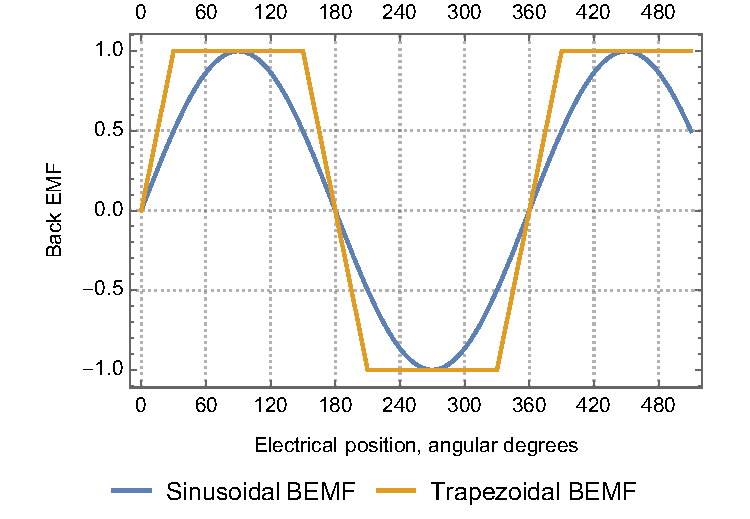
\includegraphics[width=0.6\textwidth]{bemf_trapezoidal_vs_sinusoidal}
	\caption{Difference between trapezoidal and sinusoidal BEMF.
	\label{bemf_trapezoidal_vs_sinusoidal}}
\end{figure}

Sapog, being a BLDC drive, drives the motor with trapezoidal modulated voltage.
This produces smooth torque and vibration free operation with BLDC motors,
since it is expected that the flux linkage will be changing in a specific way.

Like any BLDC drive, Sapog can operate with BLAC motors as well, albeit with increased torque ripple.
From the model presented in section \ref{sec:motor_equations} we can predict that the motor
will exhibit periodic variations in the output torque if the form of the voltage modulated by the controller
does not match with the form of the back EMF induced in the motor.
The resulting periodic torque variations that occur in a BLAC motor driven by a BLDC drive
(and, likewise, in a BLDC motor driven with sine modulated voltages) are shown on the figure 
\ref{sine_torque_deviation}.

\begin{figure}[hbt]
    \centering
	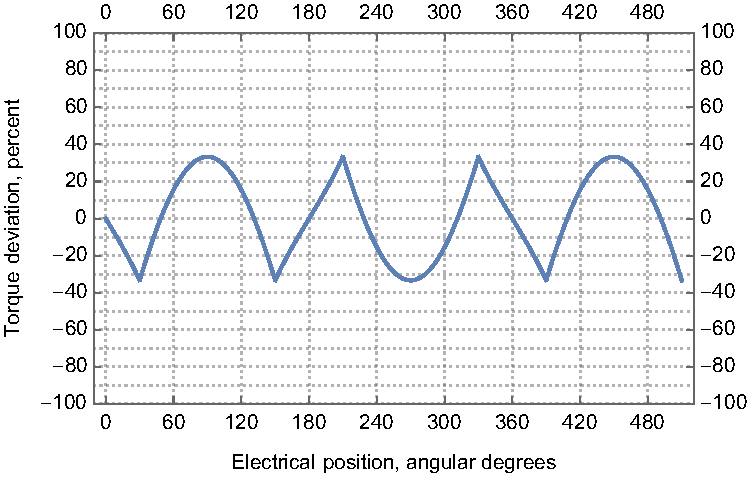
\includegraphics[width=0.6\textwidth]{sine_torque_deviation}
	\caption{Torque ripple caused by mismatching forms of the back EMF and the source voltage.
	\label{sine_torque_deviation}}
\end{figure}

Many applications, however, can tolerate the induced torque ripple and associated vibrations produced
by the motor.

\section{Motor control}

\subsection{Commutation sequence}

\newcommand{\BEMFH}{$\uparrow$}
\newcommand{\BEMFL}{$\downarrow$}

Three phase BLDC drives operate by modulating a specific sequence of voltages on the motor phases
synchronously with the movement of the rotor.
The modulated voltage sequences are shown in the commutation table below
(legend: $+$ -- positive voltage output; $-$ -- negative voltage output;
\BEMFH{} -- the phase is floating, induced BEMF is rising;
\BEMFL{} -- the phase is floating, induced BEMF is falling).

\begin{tabu}{|l c|c c c c c c|}
    \hline
    \rowfont{\bfseries}
    \multicolumn{2}{|c|}{\diagbox{Phase}{Step}}
                                 & 0     & 1     & 2     & 3     & 4     & 5     \\\hline
    \multirow{3}{*}{Forward} & A & $-$   &\BEMFH & $+$   & $+$   &\BEMFL & $-$   \\
                             & B & $+$   & $+$   &\BEMFL & $-$   & $-$   &\BEMFH \\
                             & C &\BEMFL & $-$   & $-$   &\BEMFH & $+$   & $+$   \\\hline
    \multirow{3}{*}{Reverse} & A & $-$   &\BEMFH & $+$   & $+$   &\BEMFL & $-$   \\
                             & B &\BEMFL & $-$   & $-$   &\BEMFH & $+$   & $+$   \\
                             & C & $+$   & $+$   &\BEMFL & $-$   & $-$   &\BEMFH \\\hline
\end{tabu}

The choice between forward and reverse commutation tables affects the direction of rotation of the motor,
and it is specified via the configuration parameter \CfgRef{ctl+dir}.

The rotor position is deduced from the behavior of the induced BEMF on the floating phase.
From figure \ref{bemf_trapezoidal_vs_sinusoidal} we can deduce that when the induced BEMF of the floating
phase crosses the median voltage between the high and the low phase, there is 30 electrical degrees left
before the next commutation step begins.
The controller employs this rule to estimate the time when the next commutation should occur.
The process is demonstrated on the figure \ref{commutation_basics}.
The voltage waveforms shown on the figure were acquired from the phase voltage signal conditioning circuits,
before the ADC inputs, shown on the figure \ref{power_stage_schematic}.

\begin{figure}[hbt]
    \centering
	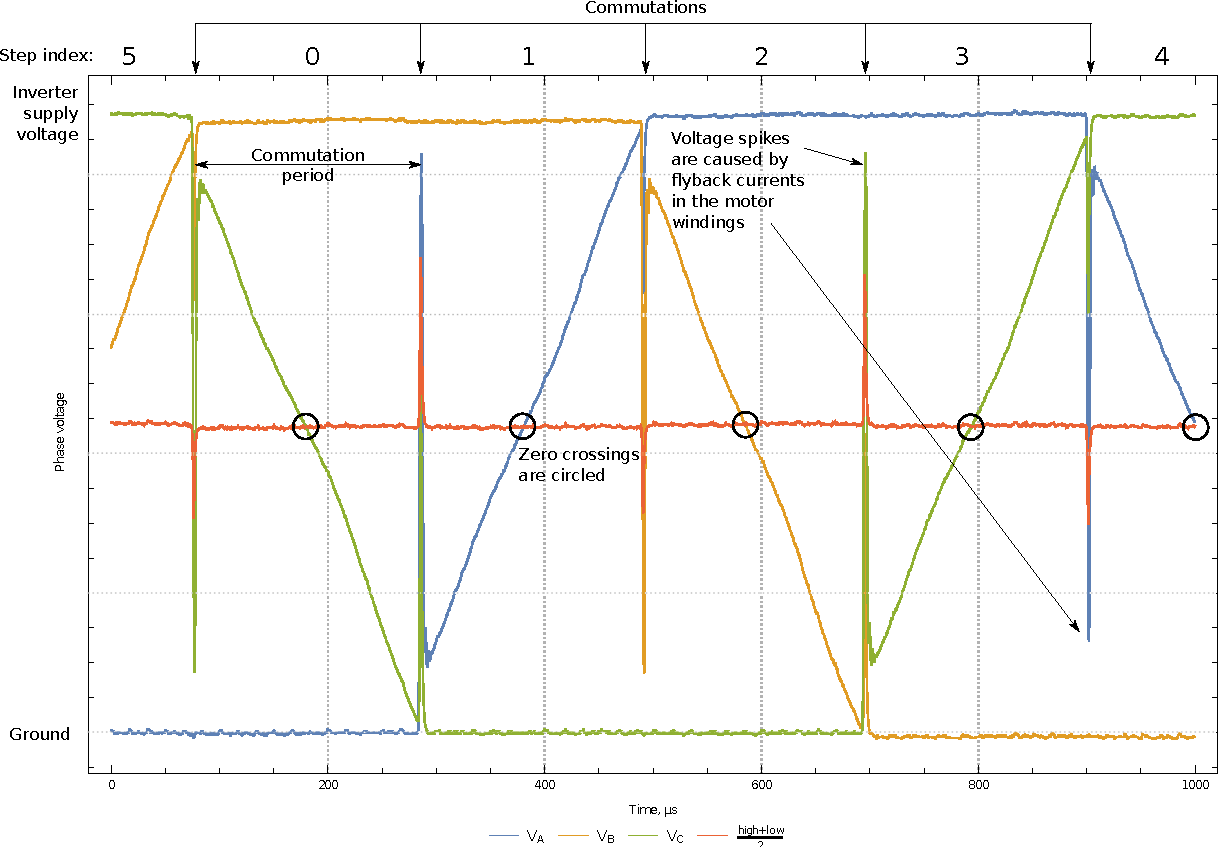
\includegraphics[width=\textwidth]{commutation_basics}
	\caption{Six step commutation sequence observed through phase voltages.
	\label{commutation_basics}}
	PWM modulation is not seen because the shown voltages were acquired while the controller
	was operating at full duty cycle.
\end{figure}

\begin{figure}[hbt]
    \centering
	
\includegraphics[width=\textwidth]{power_stage_schematic}
	\caption{Simplified schematic of the VSI and BEMF feedback circuits that Sapog relies on.
	\label{power_stage_schematic}}
\end{figure}

From the section \ref{sec:motor_equations} we know that the magnitude of the induced BEMF is linearly
dependent on the speed of relative motion between the armature and the rotor magnetic field.
Considering also the fact that the controller relies on the induced BEMF signal for rotor position estimation,
we can predict that the rotor position estimation may be unreliable if the induced BEMF is not sufficiently
strong.
In order to avoid issues at low speed operation, Sapog provides several configuration parameters that
restrict the minimum operating speed, such as the following:

\begin{itemize}
\item \CfgRef{mot+comm+per+max} - maximum commutation period, in microseconds.
The estimated commutation period will be artificially constrained to not exceed this value.
\item \CfgRef{mot+rpm+min} - minimum RPM that can be demanded in RPM governor mode.
If the demanded RPM is lower, the setpoint will be artificially increased.
\item \CfgRef{mot+v+min} - minimum source voltage when operating in open loop mode, in volts.
If the demanded duty cycle amounts to a lower source voltage than this, the setpoint will be artificially
increased.
\end{itemize}

These parameters may need adjustment to make Sapog compatible with a specific motor.
For example, if the motor cannot keep stable operation at low speed,
the minimum source voltage should be increased,
and/or the maximum commutation period should be made longer.
The minimum voltage limit does not apply to RPM loop mode,
where the minimum speed is governed by the dedicated configuration parameter shown above.

The following equation can be used to convert between commutation period $T_\text{comm}$
and electrical angular velocity $\omega_e$:
\begin{equation}
\omega_e = \frac{\pi}{3 T_\text{comm}}
\end{equation}

\subsection{Field weakening}

From section \ref{sec:motor_equations} we know that the maximum speed that a motor can achieve is dependent
on the the load, magnetic flux linkage, and the source voltage.
Reduction of the magnetic flux linkage decreases the induced BEMF, which allows the rotor reach higher speed,
given constant source voltage and load.

The controller can alter the commutation sequence in a specific way, causing the rotating magnetic field
created by the stator to interact with the magnetic field of the rotor in a way that reduces the magnetic
field linkage, effectively increasing the maximum speed of the rotor, reducing the output torque,
while keeping the maximum mechanical power output constant.
Note that since part of the energy is expended on suppression of the magnetic fields induced by the rotor,
the overall efficiency of the drive decreases with higher field weakening.

This technique is known as \emph{field weakening}, and it is implemented by means of adjustment of the 
commutation sequence, shortening the time interval from the zero crossing point to the moment when the next
commutation step begins.
In the context of BLDC drives this specific approach is also known as \emph{commutation advancing}.

Sapog defines commutation advance angle in electrical angular degrees of rotor position,
and it can vary from 0\degree{} to 29\degree{}, inclusively, where 0\degree{} corresponds to no advance,
and 29\degree{} corresponds to the maximum advance angle.
The practical effects imposed on the drive are summarized in the following table.

\begin{ZubaxCompactTable}{|c|c c c c|}
    Advance angle & Flux linkage & Maximum torque & Maximum speed & Drive efficiency \\
    Low           & High         & High           & Low           & High             \\
    High          & Low          & Low            & High          & Low              \\
\end{ZubaxCompactTable}

Sapog can modulate a fixed advance angle, or it can be defined as a function of speed.
The latter is especially useful, since high field weakening at low speeds does not make practical sense,
and serves only to reduce the drive efficiency with no apparent benefit to the application.
Additionally, high field weakening may be responsible for stability issues at low operating speeds,
because it effectively reduces the magnitude of the BEMF induced in the motor.

The field weakening feature is configured with the help of the following configuration parameters:

\begin{itemize}
\item \CfgRef{mot+tim+adv+max} - maximum commutation advance angle, in electrical rotor position degrees.
\item \CfgRef{mot+tim+adv+min} - minimum commutation advance angle, same units.
\item \CfgRef{mot+tim+cp+min} - when the current commutation period is longer than this value,
the minimum advance angle will be used. The units are microseconds.
\item \CfgRef{mot+tim+cp+max} - when the current commutation period is shorter than this value,
the maximum advance angle will be used. Same units.
\end{itemize}

When the current commutation period is between \verb|mot_tim_cp_max| and \verb|mot_tim_cp_min|,
the advance angle will be proportionally linearly interpolated between
\verb|mot_tim_adv_min| and \verb|mot_tim_adv_max|.
The interpolation logic is demonstrated on the figure \ref{timing_advance_interpolation_plot}.

\begin{figure}[hbt]
    \centering
	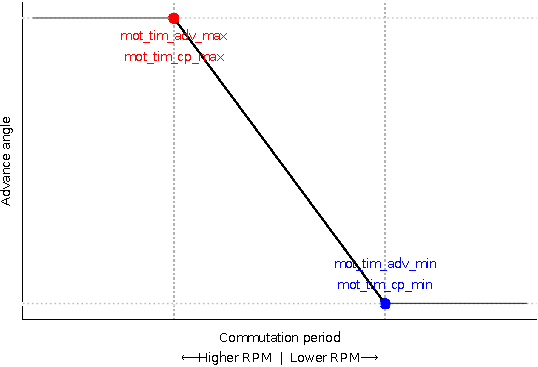
\includegraphics[width=0.6\textwidth]{timing_advance_interpolation_plot}
	\caption{Timing advance interpolation logic.
	\label{timing_advance_interpolation_plot}}
\end{figure}

Sample phase voltage waveforms acquired while the controller was operating under high field
weakening settings are shown on the figure \ref{phase_voltages_at_high_advance_angle}.

\begin{figure}[hbtp]
    \centering
	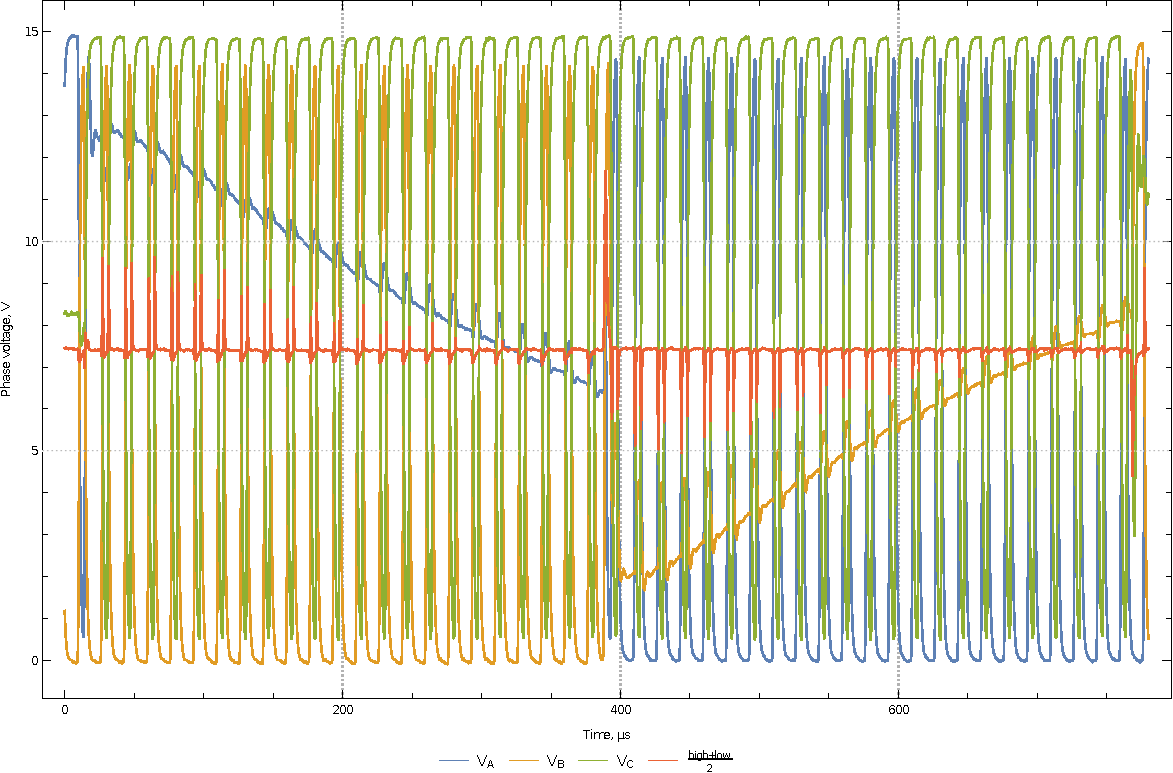
\includegraphics[width=\textwidth]{phase_voltages_at_high_advance_angle}
	\caption{Commutation sequence at high advance angle settings.
	\label{phase_voltages_at_high_advance_angle}}
	It can be seen that the next commutation begins shortly after the induced BEMF
	crosses the neutral voltage.
\end{figure}

\subsubsection{Freewheeling considerations}

Upon careful review of the field weakening effect it might become obvious that it poses certain danger
when the motor is operating at a high speed.

According to the explanations above, as long as the field weakening is active,
the controller actively suppresses the excessive flux of the permanent magnets in the rotor.
This suppression allows the controller to lower the induced BEMF, and, therefore,
extend the operating speed upwards, while keeping the source voltage constant.

Consider what happens when the inverter (or the controller as a whole) is turned off while the
motor was running with the rotor field weakened.
As the controller ceases to suppress the field, the flux linkage of the motor returns to nominal,
which, given that the speed is sufficiently high, may significantly exceed the inverter supply
voltage $V_\text{inv}$, possibly causing damage to the controller, the power supply, the motor, etc.

\subsection{Rotor position observer}

\subsubsection{BEMF processing}

As mentioned previously, Sapog deduces the current position of the rotor by tracking the induced BEMF
on the floating phase.
Which phase is floating and the direction in which BEMF is changing is dependent on the current electrical
angle of the rotor.

Measurement of the induced BEMF is done by the ADC, which is connected to the motor phases via
resistive voltage dividers which reduce the dynamic range of the motor phase voltages into a narrower
dynamic range acceptable by the ADC,
and a buffer capacitor that provides fast recharge of the sample-and-hold capacitor of the ADC,
and suppresses high frequency noise.
The resulting simplified schematic can be seen on the figure \ref{power_stage_schematic}.

BEMF measurements are sensitive to noise. In order to avoid interference with the noise generated
by the VSI, the controller synchronizes BEMF sampling with PWM switching.
However, the timing resolution provided by the resulting sampling pattern is insufficient for robust
rotor state estimation because of the sampling period restrictions imposed by the
PWM carrier frequency.

In order to work around this limitation, Sapog collects a number of samples, and,
knowing that the shape of the BEMF induced by the floating phase of a BLDC motor is linear,
solves a linear regression problem on the collected samples, effectively recovering the most likely
shape of the BEMF signal.
The resulting approximation is very robust and resilient to noise.

The principle is illustrated on the figure \ref{phase_voltage_sampling}.

\begin{figure}[hbtp]
    \centering
	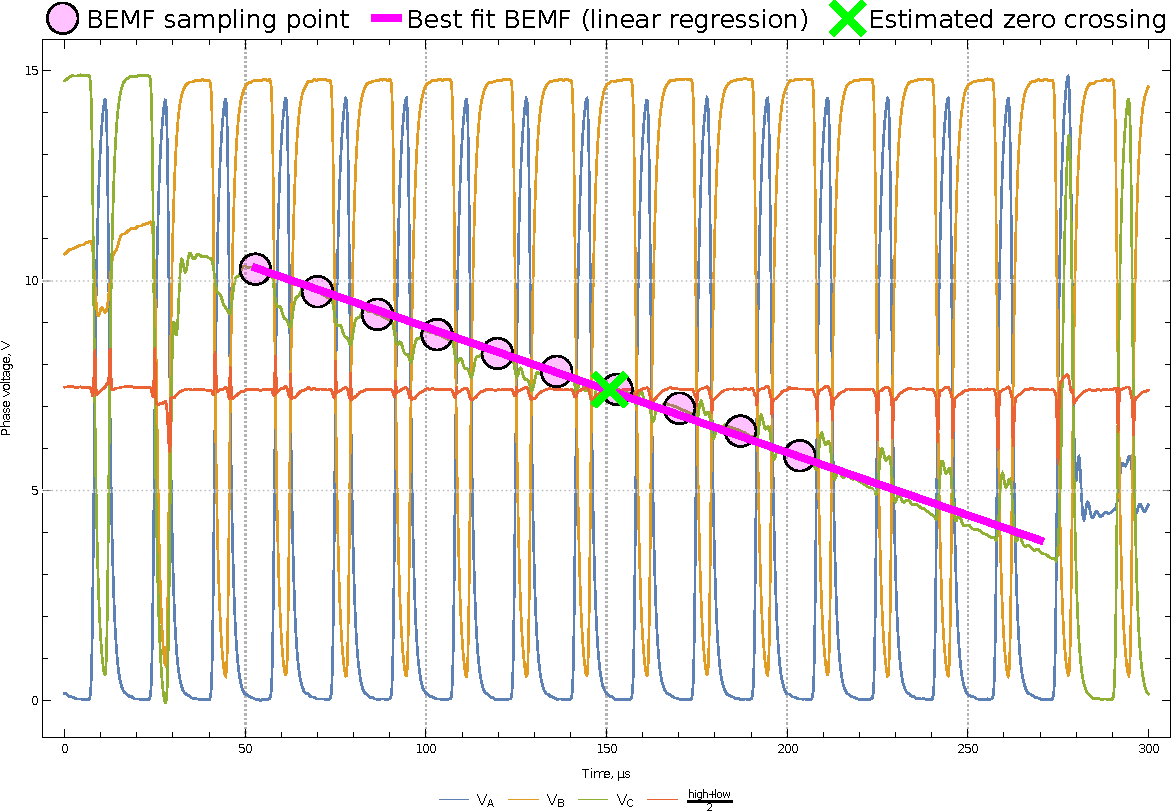
\includegraphics[width=\textwidth]{phase_voltage_sampling}
	\caption{BEMF sampling and PWM modulation.
	\label{phase_voltage_sampling}}
\end{figure}

The number of BEMF samples $N_\text{samples}$ included in the linear regression is defined by
the configuration parameter \CfgRef{mot+bemf+win+den} (dimensionless) as follows:
\begin{equation}
N_\text{samples} =
\frac{T_{\text{comm}} F_{\text{pwm}}}{\frac{\alpha\cdot\text{BWD}}{15} + \text{BWD}} + 2
\end{equation}
where $T_{\text{comm}}$ is the current commutation period,
$\text{BWD}$ is the value of the configuration parameter,
$\alpha$ is the current commutation advance angle in electrical rotor position degrees,
and $F_{\text{pwm}}$ is the PWM carrier frequency.

An attentive reader might point out that the assumption of linear BEMF that the described method rests
upon does not hold for BLAC motors, since the induced BEMF of a floating phase will be sinusoidal rather
than linear.
While the objection is correct, this deviation does not pose a significant problem, since the sinusoidal
BEMF well approximates to linear near the point of zero crossing.
Some issues may arise at very high advance angles, where the controller will be forced to resort to
look-ahead extrapolation, so that the linear regression will be applied to the sample set acquired
at the point where the linear approximation assumption does not hold.
The resulting imprecision, however, should not be of significant practical importance.

\subsubsection{Special cases}

The figure \ref{phase_voltage_sampling_corner_cases} provides a closer look at the challenges
seen by the controller in certain operating modes, which are reviewed below.

\begin{figure}[hbtp]
    \centering
	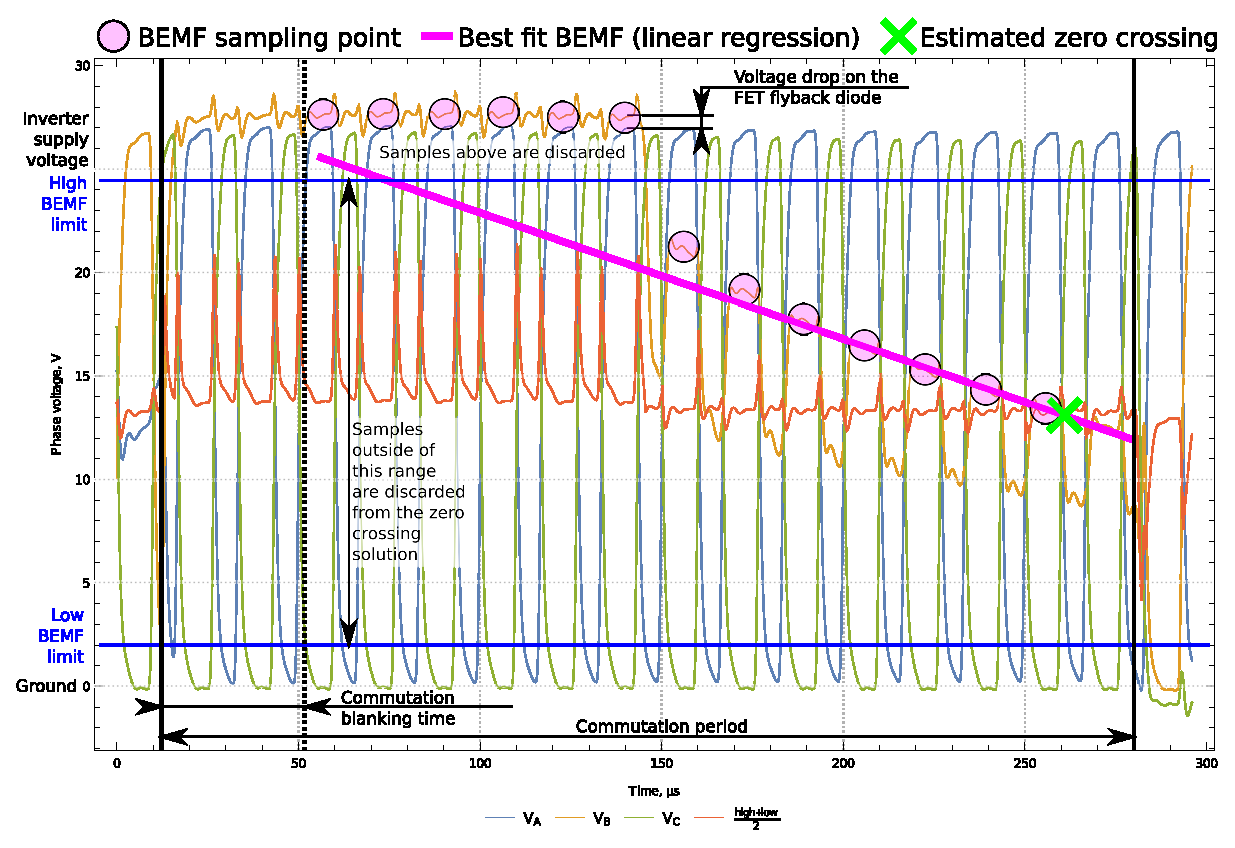
\includegraphics[width=\textwidth]{phase_voltages_braking_high_advance_angle}
	\caption{Corner cases of BEMF sampling.
	\label{phase_voltage_sampling_corner_cases}}
\end{figure}

In certain operating modes the induced BEMF of the floating phase may briefly exceed the
inverter supply voltage $V_\text{inv}$, or fall below the ground level,
causing voltage drop on either the high-side or low-side flyback diodes, respectively.
BEMF samples acquired at this time are not representative of the true form of the signal,
because the signal is altered by external factors;
and therefore, such samples cannot be used for the linear regression.
Sapog uses a simple heuristic that allows it to detect when the sampled signal is subjected to
altering and discard the affected samples.
The heuristic checks whether the sampled voltage falls into a specified range near the neutral voltage,
and discards the sample if it doesn't.

Additionally, samples acquired shortly after commutation may be subjected to transient distortions.
Sapog works around that by imposing a fixed \emph{blanking time} after a commutation, during which
BEMF sampling is not performed.

The following configuration parameters are relevant to the reviewed aspects:

\begin{itemize}
\item \CfgRef{mot+bemf+range} - the voltage range around neutral,
in percent of the inverter supply voltage $V_\text{inv}$, where the BEMF samples
will be considered valid and accepted into the solution.
\item \CfgRef{mot+blank+usec} - duration of the blanking time after the commutation, in microseconds.
\end{itemize}

Additional difficulties are posed by operation at very high power levels,
and/or when the controlled motor exhibits high inductance of the windings.
Under these conditions, the motor windings tend to accumulate significant energy during the duration
of the commutation period.
When the current commutation period ends, the winding is released, but the accumulated energy maintains
some current through the winding and the \emph{flyback diode} of one of the transistors until
the energy is dissipated.
This current caused by the energy release from a disconnected inductive network is known as
\emph{flyback current}.
As long as the flyback current is flowing though the winding and the flyback diode,
the induced BEMF is completely suppressed and, therefore,
is unobservable, which does not allow the controller to evaluate the state of the rotor.

\begin{figure}[hbtp]
    \centering
	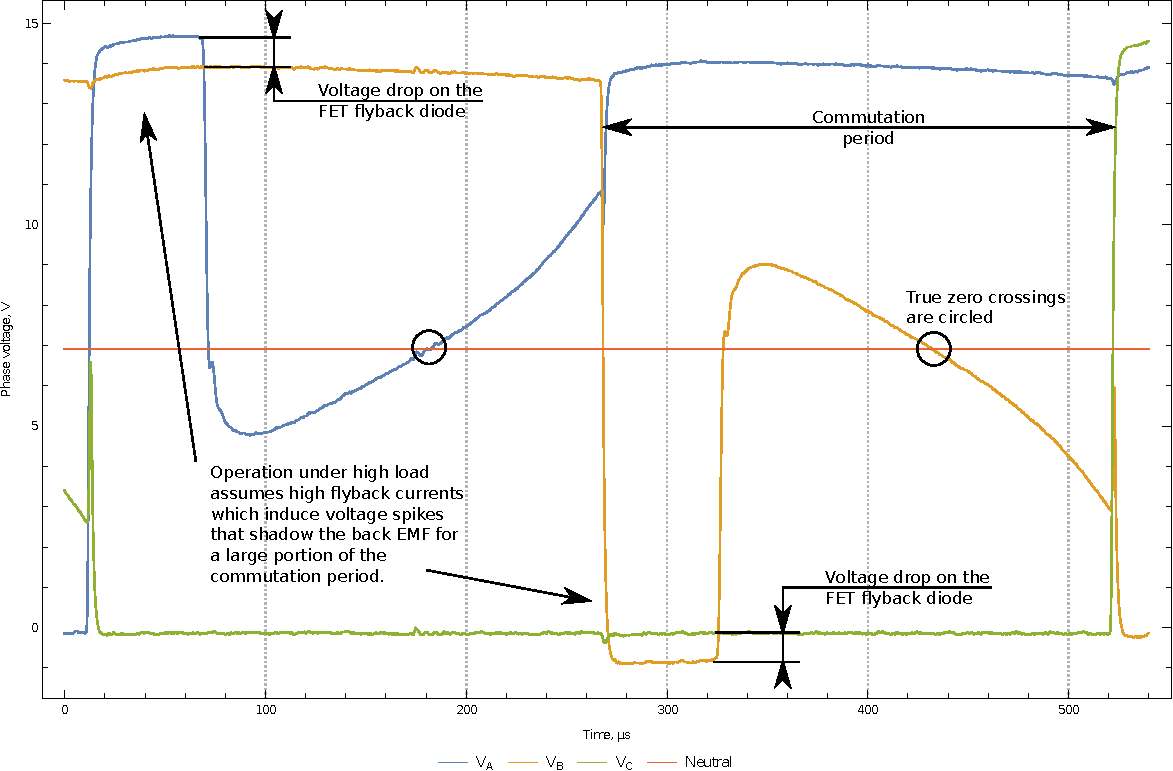
\includegraphics[width=\textwidth]{phase_voltages_at_high_load}
	\caption{Challenges of high power operation.
	\label{phase_voltages_at_high_load}}
\end{figure}

Sapog recognizes this condition and waits for the flyback current to cease.
If the current is still flowing past a certain deadline necessary for the controller to evaluate the
point of zero crossing, Sapog enters a \emph{desaturation mode} in order to bring the system
back into observable state.
In the desaturation mode Sapog turns off the inverter and waits until the next commutation period.
By the time the next commutation period begins, the flyback currents will have ended,
allowing the controller to continue observation of the motor state.

The figure \ref{phase_voltages_at_high_load} shows operation near the point of activation
of the desaturation mode.

\subsubsection{Maximum speed restrictions}

It is easy to see that as the speed increases and the commutation period shortens,
the number of BEMF samples that can be accommodated within the commutation period will be decreasing.
This effect imposes the limit on the maximum achievable speed, and the limit is dependent on the PWM
carrier frequency.

When the drive operates in open loop mode, the controller will limit the maximum duty cycle
when the commutation period reaches dangerously low values.
The limiting is done by means of a simple P-controller,
which begins to override the duty cycle setpoint when it exceeds a certain value.

When the drive operates in RPM control loop mode, the limiting will be performed simply by means of
clipping the RPM setpoint.

The exact thresholds are specified on the figure \ref{pwm_maximum_speed}.

The configuration parameter \CfgRef{mot+pwm+hz} can be used to set the desirable PWM frequency
in hertz.
It is recommended to keep the frequency as low as possible,
as that would facilitate lower switching losses and therefore higher efficiency of the drive.

\begin{figure}[hbt]
    \centering
	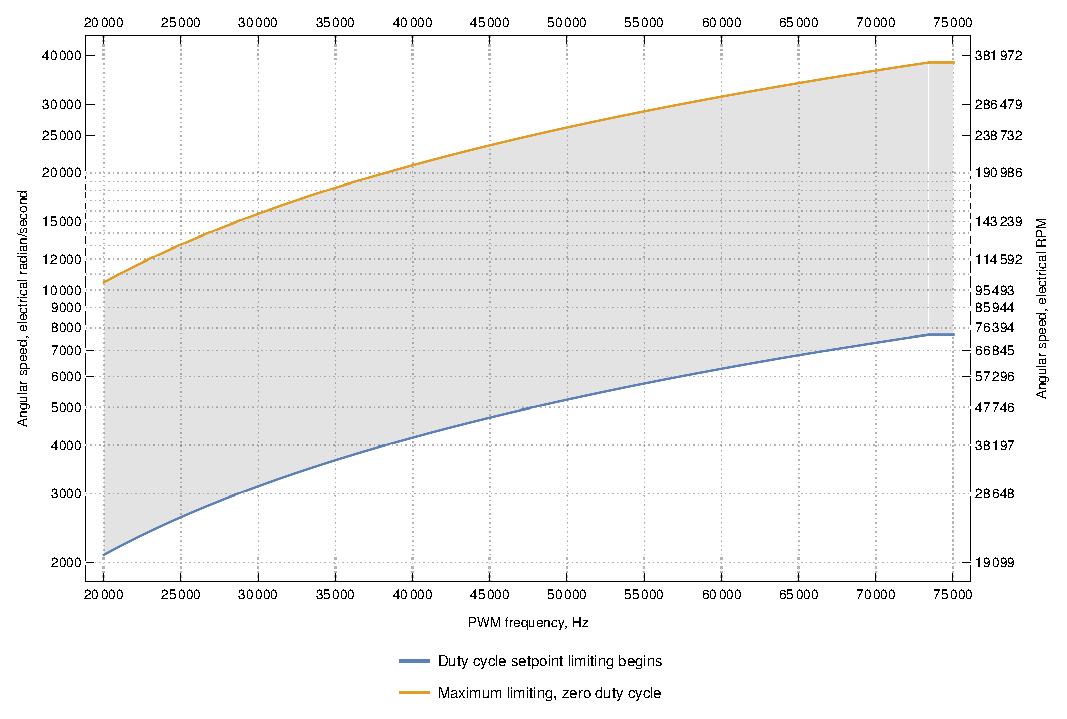
\includegraphics[width=\textwidth]{pwm_maximum_speed}
	\caption{Dependency of the maximum speed on PWM frequency.
	\label{pwm_maximum_speed}}
\end{figure}

\subsubsection{Field weakening restrictions}

The controller requires several microseconds to solve the linear regression problem after the sampling is
finished.
However, operation at very high advance angles requires the controller to perform commutation virtually
immediately after the zero crossing has happened, leaving very little time to perform the computation.
The controller strives to work around this contradiction by trying to robustly extrapolate the shape of the
BEMF signal, predicting the upcoming zero crossing ahead of time.

Despite that, operation at very high speeds may not provide the time necessary to take a sufficient
number of samples and solve the regression problem before the next commutation is due.
In this case, Sapog will silently lower the current advance angle and keep it at as close to the requested
value as the current operating mode permits.

\subsection{Regenerative braking}



\subsection{Rotor stall detection}



\subsection{Spin-up}

\begin{figure}[hbt]
    \centering
	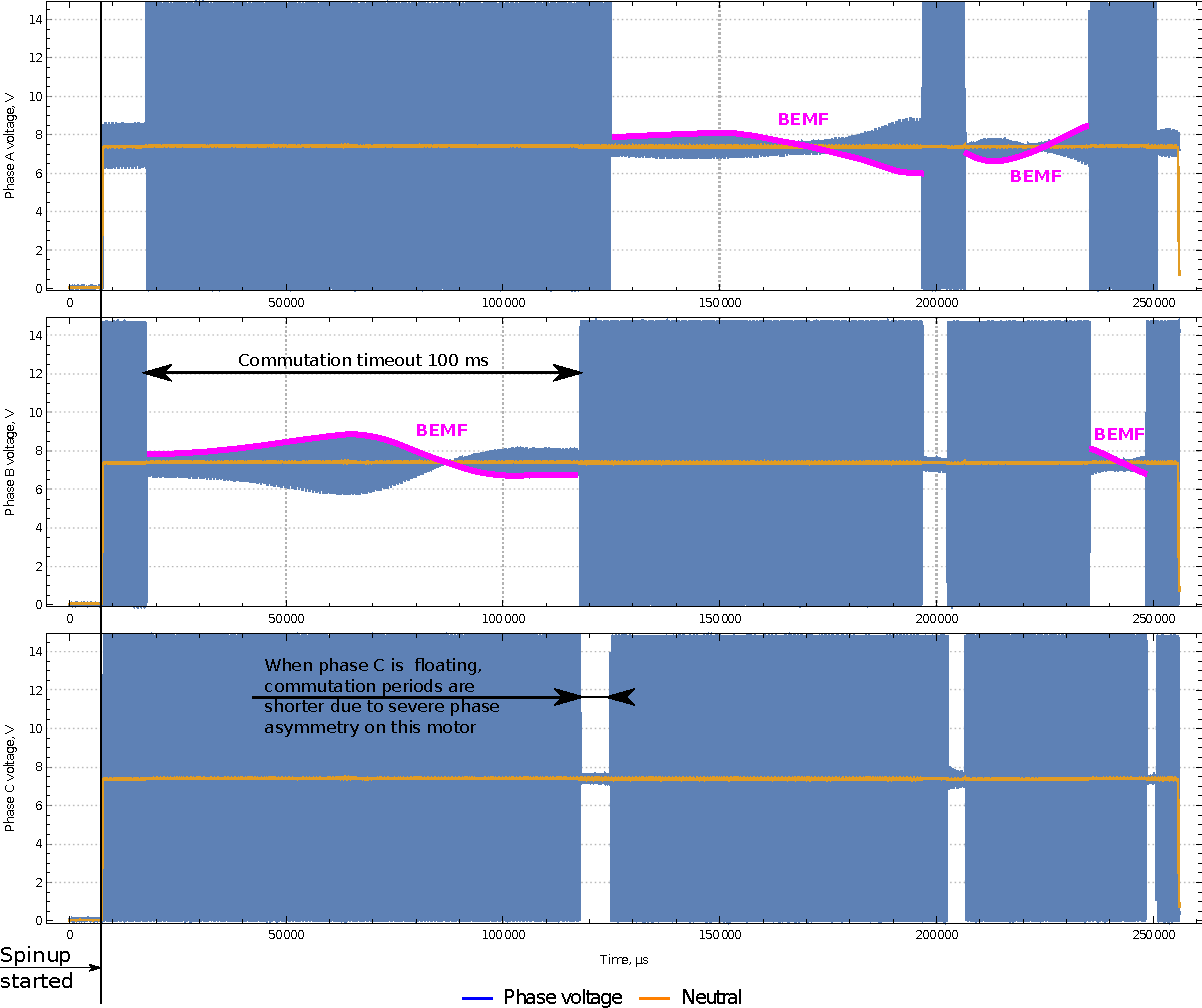
\includegraphics[width=\textwidth]{spinup_phase_voltages}
	\caption{Spin-up sequence with a highly inertial load.
	\label{spinup_phase_voltages}}
\end{figure}

\subsection{Open loop operation}



\subsection{RPM control loop}

TODO provide exact units of the configuration parameters.

\subsection{Current measurement}



\section{Self diagnostics}



\chapter{Configuration parameters}

\CfgDef{esc+index}
\CfgDef{cmd+ttl+ms}
\CfgDef{cmd+start+dc}
\CfgDef{uavcan+node+id}
\CfgDef{light+index}
\CfgDef{pwm+max+usec}
\CfgDef{pwm+min+usec}
\CfgDef{pwm+enable}
\CfgDef{enum+max+step}
\CfgDef{enum+steps}
\CfgDef{enum+bemf}
\CfgDef{mot+pwm+dt+ns}
\CfgDef{mot+pwm+hz}
\CfgDef{mot+spup+blnk+pm}
\CfgDef{mot+spup+to+ms}
\CfgDef{mot+spup+st+cp}
\CfgDef{mot+comm+per+max}
\CfgDef{mot+zc+fails+max}
\CfgDef{mot+bemf+range}
\CfgDef{mot+bemf+win+den}
\CfgDef{mot+blank+usec}
\CfgDef{mot+tim+cp+min}
\CfgDef{mot+tim+cp+max}
\CfgDef{mot+tim+adv+max}
\CfgDef{mot+tim+adv+min}
\CfgDef{mot+i+shunt+mr}
\CfgDef{rpmctl+i}
\CfgDef{rpmctl+d}
\CfgDef{rpmctl+p}
\CfgDef{mot+stop+thres}
\CfgDef{mot+lpf+freq}
\CfgDef{mot+i+max+p}
\CfgDef{mot+i+max}
\CfgDef{mot+rpm+min}
\CfgDef{ctl+dir}
\CfgDef{mot+num+poles}
\CfgDef{mot+dc+slope}
\CfgDef{mot+dc+accel}
\CfgDef{mot+spup+vramp+t}
\CfgDef{mot+v+spinup}
\CfgDef{mot+v+min}

\end{document}
